\chapter{Administrator manual}
\label{chap:admin}

The following administrator manual requires some enhanced knowledge about
\begin{itemize}
\item Linux/Ubuntu
\item Network configuration
\item Source code management with git
\item ROS installation and usage
\end{itemize}
If you are missing some of this requirements or feel uncomfortable with what you are doing, please interrupt and ask somebody to help you before continuing.

%#################################################################################################
\section{Setup robot pcs}
%#################################################################################################
On all Care-O-bots there are at least two pcs. Some Care-O-bots have an optional third pc, which is not covered by this manual. Within this section we will guide you through setting up new pcs. When nothing otherwise is mentioned the following instructions are for both pc1 and pc2, please do the same steps on both pcs.

To pc1 all actuators are connected, sensors are connected both, to pc1 and pc2. All camera sensors are connected to pc2, whereas all other sensors like e.g. laser scanners are connected to pc1. By default pc3 is not connected to any hardware and therefore can be used as additional computing power.

\subsection{Install operating system}
The first step is to install the operating system for each pc, which means pc1 and pc2 (optionally pc3). We are using Ubuntu as the main operating system for the robot. We recommend to install the \textbf{Ubuntu 14.04 LTS (long term stable) 64-bit} version because this version is well tested to work with the hardware. 

First please install Ubuntu (English version) creating a normal swap partition. Please choose \texttt{robot} as an admin account with a really safe password which should only be known to the local robot administrator. The hostname of the pc should be \texttt{cob3-X-pc1} and \texttt{cob3-X-pc2}.
\abbrev{X}{Robot configuration number}

\subsection{Setup internal robot network}\label{sec:network}
Inside the robot there's a router which connects the pcs and acts as gateway to the building network. Setup the router with the following configuration. 

The ip address of the router should be \texttt{192.168.IP.1} and for the internal network dhcp should be activated. Use \texttt{cob3-X} as hostname for the router. Register the MAC addresses of pc1 and pc2 so that they get a fixed ip address over dhcp. Use \texttt{192.168.IP.101} for pc1 and \texttt{192.168.IP.102} for pc2. Enable portforwarding for port \texttt{2201} to \texttt{192.168.IP.101} and for port \texttt{2202} to \texttt{192.168.IP.102}, where IP parameter is defined depending on the robot \ref{IP_table}.

\begin{table}[h]
\begin{center}
\begin{tabular}{ | l | c | }
  \hline
  cob3-X & IP=X \\
  \hline
  raw3-X & IP=40+X \\
  \hline
  desire & IP=100 \\
  \hline
\end{tabular}
\end{center}
\caption{IP address definition}
\label{IP_table}
\end{table}

After ensuring that the network configuration of the router is setup correctly, we can configure the pcs. All pcs should have two Ethernet ports. The upper one should be connected to the internal router. 

\subsection{Install basic setup}
Next we have to install some basic tools for the further setup of the pcs. In order to install the packages a internet connection is needed.

The full Care-O-bot installation can be done using a bash script. The script is in the setup repository, get it using the following command:

\begin{lstlisting}
wget https://raw.githubusercontent.com/ipa320/setup/master/InstallCob3.sh
chmod +x InstallCob.sh
\end{lstlisting}


The installation script needs the parameters robot, ip address and installation mode, where:
\begin{itemize}
\item -r robot: is the robot name (cob3-X)
\item -ip :ip address for your actual installation pc, use \texttt{192.168.IP.101} for pc1 and \texttt{192.168.IP.102} for pc2, if you have  a third pc, assign it the ip \texttt{192.168.IP.103}
\item -m installation mode: on Care-O-bot there are two different types of computers, the master pc and the slave. The master PC has a large hard disk , and works as a NFS system server, the other computers will be the clients
\end{itemize}

The script allow different types of installation:

\begin{enumerate}
\item \texttt{Basic Installation} It is composed by the following steps:
\begin{itemize}
\item Install basic tools (vim, meld, terminator ...)
\item Install and configure openssh
\item Allow robot user to execute sudo command without password
\item Setup root user (in this step the user will be asked for a password)
\item Install ROS
\item Setup udev rules
\item Setup bash environment 
\end{itemize}
\item \texttt{Setup NTP and NFS} This option will configure the NFS system depending on the installation mode, it is important that the master pc is already installed and per network reachable before install the slave computers, otherwise the installation process will be cancelled. After this installation it is necessary restart the computer.
\item \texttt{Full Installation} A full installation means the combination of 1 and 2 (Basic Installation + Setup NTP and NFS)
\item \texttt{Cob setup} This step holds the recommended configuration of the robot home directory. This step can only be execute after a full installation.
\end{enumerate}

After the network is configured properly we can setup a NFS between the robot pcs. pc2 will act as the NFS server and pc1 as NFS client, start always the installation with the master pc, in this case \texttt{cob3-X-pc2}

Run the Install script on pc2:
\begin{lstlisting}
./InstallCob3.sh -r cob3-X -ip 192.168.X.102 -m master
\end{lstlisting}

Please take your time to check that the given parameters are right before continue, after the verification choose the option 3 (Full installation). The installation will take around 30 minutes , depending on the internet connection. During the process the user will be asked to confirm and verify the selected options. 

After the successfully pc2 installation and with all the computers connected to the router, repeat the process with the client pcs (cob3-X-pc1):

\begin{lstlisting}
./InstallCob3.sh -r cob3-X -ip 192.168.X.101 -m slave
\end{lstlisting}

After the full installation of all the Care-O-bot computers, the home directory can be configured calling the Install script again on master pc (cob3-X-pc2):
Run the Install script on pc2:
\begin{lstlisting}
./InstallCob3.sh -r cob3-X -ip 192.168.X.102 -m master
\end{lstlisting}

And choose the option 4 (Cob setup).

\subsection{Setup hardware components}
In order to use the different hardware components we have to install the drivers and set permission rights. All hardware configuration is stored in the \texttt{cob\_hardware\_config} package.

\paragraph{Setup can bus drivers}
This step is necessary for all drivers with can bus interface (Schunk powercubes, Schunk sdh, head axis, base). In general both can drivers from Peak Systems\footnote{\url{http://www.peak-system.com/}} \texttt{libpcan} and ESD\footnote{\url{http://www.esd-electronics.com}} \texttt{libntcan} can be used. Installation instructions can be found in the package documentation of libpcan \url{http://www.ros.org/wiki/libpcan} and libntcan \url{http://www.ros.org/wiki/libntcan}.

\subsubsection{Scanners}

\paragraph{Sick S300 laser scanners}
The Sick S300 scanners on the front side and backside of the robot are connected via USB to pc1. Configuration is done in the \texttt{cob\_hardware\_config} package in \texttt{config/laser\_front.yaml} and \texttt{config/laser\_rear.yaml}, documentation about parameters in \footnote{\url{http://www.ros.org/wiki/cob_sick_s300}}.

To receive data from the Sick S300 scanners check if the user is in the \texttt{dialout} group
\begin{lstlisting}
groups
\end{lstlisting}

For testing you can run the front laser scanner with
\begin{lstlisting}
roslaunch cob_bringup sick_s300.launch name:=front
\end{lstlisting}

To check if there is some data published use
\begin{lstlisting}
rostopic hz /scan_front
\end{lstlisting}

Check the rear scanner in the same way, the argument name is rear ( \texttt{name:=rear} ) and the topic \texttt{/scan\_rear}.

You have to configurate the scanners and setup the safety region for each scanner. It can be done using the Sick CDS software \footnote{\url{http://www.sick.com/group/EN/home/service/software/Pages/configurationsoftwarecds.aspx}}.

\textbf{Note on new firmware (2.10 and greater):} 
Sick changed their scanner product line. From now on (April 2013) the Sick Professional CMS, that we used so far, has been replaced by the Sick Expert.
The main difference is, that there is now no additional CMS version anymore.
Expert equals to CMS, whereas Professional no longer has the CMS capabilities.
The new scanners are also shipped with a new firmware (2.10).
It is thus not possible anymore, to simply flash an old configuration as it might break the scanner.
Additionally, the new scanners also have a new telegram protocol version, which is not compatible with the current driver.
However, it can be configured to use the old protocol versions.
How to setup the scanner with the new firmware is described in the following.

\textbf{How to setup Sick laser scanners with firmware version 2.10:}
Make sure you have CDS 3.6.7 installed (even though it is not the latest one, this is the recommended version from the Sick support).
When the scanner is connected and the CDS has started, add a new device to the respective COM port (do NOT hit the \texttt{Recognize Project} button).
Choose the correct device: S300 Expert (CMS should be entered automatically).
Check the \texttt{Compatibility Mode} box; this serves to enable the old telegram protocoll version.
After that you can edit the configuration or import one (the current configurations for the scanners can be found in the robot specific folders on GitHub\footnote{\url{https://github.com/ipa320/setup/tree/master/backup_configuration}}, \texttt{raw3-3} contains configurations for the new scanners).
If you are not sure which scanner your robot has, have a look at the distribution site on ros.org\footnote{\url{http://www.ros.org/wiki/Robots/Care-O-bot/distribution}}.

\textbf{Note on importing scanner fields:}
Please note that even though you can easily export and import any configurations, the scanner fields are not contained in the configuration files.
You need to export and import the scanner fields separately using the CDS.
This can be done in the \texttt{File} menu.

We recommend the following configuration:
\begin{itemize}
\item System parameters:
\begin{itemize}
\item Aplication name: COB3
\item Device name S300[H]: S300-V
\item Device name S300[G]: S300-H
\item Name of the user: IPA
\end{itemize}
\item Resolution/scanning range:
\begin{itemize}
\item Aplication: Mobile
\item Resolution: 30 mm
\end{itemize}
\item Restart:
\begin{itemize}
\item Time delayed by: 2 Seconds
\end{itemize}
\item Field sets:
\\
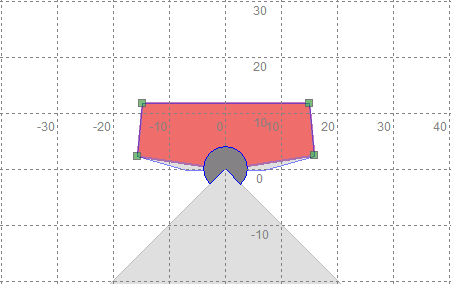
\includegraphics[width=0.65\textwidth]{images/area.png}
\\ The safety region should have 4 points:
\begin{itemize}
\item x=15 cm y=12 cm
\item x=-15 cm y=12 cm
\item x$\approx$15 cm y$\approx$2.5 cm (depend on the cover)
\item x$\approx$-15 cm y$\approx$2.5 cm (depend on the cover)
\end{itemize}
\item Measure data output:
\begin{itemize}
\item Baud rate: 500 kBaud
\item Send mode: Continuous data output
\item Measured data output: Distance
\item Beginning: -45
\item End: 225
\end{itemize}
\end{itemize}

\paragraph{Hokuyo URG laser scanner}
The Hokuyo laser scanner is connected to PC1 via USB. The configuration of this device is defined in the launch file as parameters \texttt{cob\_bringup/components/laser\_top.launch}.

For testing the scanner you have to call the run the node:
\begin{lstlisting}
rostlaunch cob_bringup hokuyo.launch name:=top
\end{lstlisting}

You can check the output of the topic:
\begin{lstlisting}
rostopic hz /scan_top
\end{lstlisting}

\subsubsection{Base}

\paragraph{Relayboard}
The Relayboard is connected to PC1 via USB. The configuration file (\texttt{relayboard.yaml}) is in the package \texttt{cob\_hardware\_config} inside the folder \texttt{cob3-X/config}.

For testing the Relayboard you have to launch the file:
\begin{lstlisting}
roslaunch cob_bringup relayboard.launch
\end{lstlisting}

And checking the output of the topic \texttt{/emergency\_stop\_state} prove its correct operation:
\begin{lstlisting}
rostopic echo /emergency_stop_state
\end{lstlisting}

\paragraph{Base}
You have to configure the elmo controllers, all the information about the driver is in \footnote{\url{http://www.ros.org/wiki/cob_base_drive_chain}}, you find the parameters of this configuration in \texttt{cob\_hardware\_config} package in \texttt{cob3-X/config/base}.

For testing you can launch the base with:
\begin{lstlisting}
roslaunch cob_bringup base_solo.launch
\end{lstlisting}
Init the component using the service:
\begin{lstlisting}
rosservice call /base_controller/init
\end{lstlisting}
And try to move the base using the joystick \ref{subsec:joystick}

\subsubsection{Torso}
\paragraph{Torso with PRL modules}
There are two parts where configuration needs to be set. One part of the configuration is done inside the firmware of the powercubes and the other one is done through ROS parameters.

First make sure that the powercube settings in the firmware are correct. You can see and modify the parameters using the windows based PowerCubeCtrl software from the schunk homepage\footnote{\url{http://www.schunk-modular-robotics.com/left-navigation/service-robotics/service-download/software/prl/powercube.html}}. A sample configuration can be fount at \footnote{\url{tbd}}.

The ROS configuration is done in \texttt{cob\_hardware\_config}, in \texttt{cob3-X/config/torso.yaml}. Documentation about the ROS parameters can be found at \footnote{\url{http://www.ros.org/wiki/schunk_powercube_chain}} and \footnote{\url{http://www.ros.org/wiki/cob_trajectory_controller}}.

There is a launch file in cob\_bringup per driver for testing:

\begin{lstlisting}
roslaunch cob_bringup component_solo_basics.launch
roslaunch cob_bringup schunk_powercube_chain_driver.launch component_name:=torso
\end{lstlisting}

For initialing and moving you can use the cob\_command\_gui \ref{subsec:command_gui}.

These components should be manual calibrated as it is explained on \ref{sec:manual_calibration}.

\paragraph{Torso with PRL-plus modules}

There are two parts where configuration needs to be set. One part of the configuration is done inside the firmware of the MTS and the other one is done through ROS parameters.

First make sure that the MTS settings in the firmware are correct. You can see and modify the parameters using the windows based MTS software from the schunk homepage \footnote{\url{http://www.de.schunk.com/schunk/schunk_websites/service/download_tracking.html?href=MTS_v_1_56_20130904.zip&country=DEU&lngCode=DE&lngCode2=DE}}. A sample configuration can be fount at \footnote{\url{tbd}}.

The ROS configuration is done in \texttt{cob\_hardware\_config}, in \texttt{cob3-X/config/torso\_controller.yaml}, \texttt{cob3-X/config/torso\_driver.yaml} and \texttt{cob3-X/config/canX.yaml}. Documentation about the ROS parameters can be found at \footnote{\url{http://wiki.ros.org/ros_canopen}}.


There is a launch file in cob\_bringup per driver for testing:

\begin{lstlisting}
roslaunch cob_bringup component_solo_canopen.launch component_name:=torso can_module:=canX
\end{lstlisting}

For initiating and moving you can use the cob\_command\_gui \ref{subsec:command_gui}.

These components should be manual calibrated as it is explained on \ref{sec:manual_calibration}.

\subsubsection{Trays}
\paragraph{One DOF tray with PRL modules}

There are two parts where configuration needs to be set. One part of the configuration is done inside the firmware of the Powercubes and the other one is done through ROS parameters.

First make sure that the powercube settings in the firmware are correct. You can see and modify the parameters using the windows based PowerCubeCtrl software from the schunk homepage\footnote{\url{http://www.schunk-modular-robotics.com/left-navigation/service-robotics/service-download/software/prl/powercube.html}}. A sample configuration can be fount at \footnote{\url{tbd}}.

The ROS configuration is done in \texttt{cob\_hardware\_config}, in \texttt{cob3-X/config/tray.yaml}. Documentation about the ROS parameters can be found at \footnote{\url{http://www.ros.org/wiki/schunk_powercube_chain}} and \footnote{\url{http://www.ros.org/wiki/cob_trajectory_controller}}.

There is a launch file in cob\_bringup per Schunk component for testing:

\begin{lstlisting}
roslaunch cob_bringup component_solo_basics.launch
roslaunch cob_bringup schunk_powercube_chain_driver.launch component_name:=tray
\end{lstlisting}

For initialing and moving you can use the cob\_command\_gui \ref{subsec:command_gui}.

These components should be manual calibrated as it is explained on \ref{sec:manual_calibration}.

\paragraph{3 DOF tray and one DOF tray with PRL-plus modules}

There are two parts where configuration needs to be set. One part of the configuration is done inside the firmware of the MTS and the other one is done through ROS parameters.

First make sure that the MTS settings in the firmware are correct. You can see and modify the parameters using the windows based MTS software from the schunk homepage\footnote{\url{http://www.de.schunk.com/schunk/schunk_websites/service/download_tracking.html?href=MTS_v_1_56_20130904.zip&country=DEU&lngCode=DE&lngCode2=DE}}. A sample configuration can be fount at \footnote{\url{tbd}}.

The ROS configuration is done in \texttt{cob\_hardware\_config}, in \texttt{cob3-X/config/tray\_controller.yaml}, \texttt{cob3-X/config/tray\_driver.yaml} and \texttt{cob3-X/config/canX.yaml}. Documentation about the ROS parameters can be found at \footnote{\url{http://wiki.ros.org/ros_canopen}}.


There is a launch file in cob\_bringup per driver for testing:

\begin{lstlisting}
roslaunch cob_bringup component_solo_canopen.launch component_name:=tray can_module:=canX
\end{lstlisting}

For initiating and moving you can use the cob\_command\_gui \ref{subsec:command_gui}.

These components should be manual calibrated as it is explained on \ref{sec:manual_calibration}.

\subsubsection{Arms}


\paragraph{Schunk powercubes LWA}
There are two parts where configuration needs to be set. One part of the configuration is done inside the firmware of the powercubes and the other one is done through ROS parameters.

First make sure that the powercube settings in the firmware are correct. You can see and modify the parameters using the windows based PowerCubeCtrl software from the schunk homepage\footnote{\url{http://www.schunk-modular-robotics.com/left-navigation/service-robotics/service-download/software/prl/powercube.html}}. A sample configuration can be fount at \footnote{\url{tbd}}.

The ROS configuration is done in \texttt{cob\_hardware\_config}, in \texttt{cob3-X/config/lwa.yaml} or \texttt{/config/torso.yaml}. Documentation about the ROS parameters can be found at \footnote{\url{http://www.ros.org/wiki/schunk_powercube_chain}} and \footnote{\url{http://www.ros.org/wiki/cob_trajectory_controller}}.

There is a launch file in cob\_bringup per schunk component for testing:

\begin{lstlisting}
roslaunch cob_bringup lwa_solo.launch
\end{lstlisting}

For initialing and moving you can use the cob\_command\_gui \ref{subsec:command_gui}.

These components should be manual calibrated as it is explained on \ref{sec:manual_calibration}.

\paragraph{Schunk powercubes LWA4D}

There are two parts where configuration needs to be set. One part of the configuration is done inside the firmware of the MTS and the other one is done through ROS parameters.

First make sure that the MTS settings in the firmware are correct. You can see and modify the parameters using the windows based MTS software from the schunk homepage\footnote{\url{http://www.de.schunk.com/schunk/schunk_websites/service/download_tracking.html?href=MTS_v_1_56_20130904.zip&country=DEU&lngCode=DE&lngCode2=DE}}. A sample configuration can be fount at \footnote{\url{tbd}}.

The ROS configuration is done in \texttt{cob\_hardware\_config}, in \texttt{cob3-X/config/arm\_controller.yaml}, \texttt{cob3-X/config/arm\_driver.yaml} and \texttt{cob3-X/config/canX.yaml}. Documentation about the ROS parameters can be found at \footnote{\url{http://wiki.ros.org/ros_canopen}}.


There is a launch file in cob\_bringup per driver for testing, for the canopen the can port where it is connected has to be given as argument:

\begin{lstlisting}
roslaunch cob_bringup component_solo_canopen.launch component_name:=arm can_module:=canX
\end{lstlisting}

For initiating and moving you can use the cob\_command\_gui \ref{subsec:command_gui}.

These components should be manual calibrated as it is explained on \ref{sec:manual_calibration}.

\paragraph{KUKA LBR}
The Kuka LBR PC is connected to PC1 by Ethernet cable, you have to configure the IP address adding to the file /etc/network/interfaces the following lines:
\begin{lstlisting}
auto eth1
iface eth1 inet static
address 192.168.42.15
netmask 255.255.255.0
\end{lstlisting}

You can also give the alias name (lbr\_box) to the arm ip address, adding the this line to /etc/hosts:
\begin{lstlisting}
192.168.42.146  lbr_box
\end{lstlisting}

You have to compile the cob\_lbr repository (this repository is not public, please ask us for it) :
\begin{lstlisting}
rosmake cob_lbr
\end{lstlisting}

For testing , the first step is check the connection with the arm PC:
\begin{lstlisting}
ping 192.168.42.146
ping lbr_box
\end{lstlisting}

The initialization process for LBR is done through the lbr\_box, you can login from PC1 to the lbr\_box via telnet:
\begin{lstlisting}
telnet lbr_box
\end{lstlisting}

Now you can initialize the LBR, therefore type: 
\begin{lstlisting}
<l
\end{lstlisting}

in the telnet terminal and wait for the line ”Stable state RUNNING reached!”. If you don’t see this line, contact your robot administrator: there’s possibly something wrong.
For a correct operation of the LBR it is important that the controller gets to know both states, emergency stop active and released. Therefore activate the emergency stop for about 15 seconds until you see ”administrationThread emerg change 1 0”. After releasing the emergency stop again you should see ”administrationThread emerg change 0 1”.
To lougout from telnet use Ctrl+D.

Now you can bringup the LBR with the command:
\begin{lstlisting}
roslaunch cob_bringup lbr.launch
\end{lstlisting}

For moving you can use the cob\_command\_gui \ref{subsec:command_gui}.

\paragraph{Universal Robot 5}

The arm with universal robot manipulator has 2 components the universal robot and a connector. This connector is managed by ipa\_canopen package \ref{ipacanopen}.

TODO: configure the module with the windows software
TODO: config files (cob\_hardware\_config)  ur\_connector\_canopenmaster.yaml and ur\_connector.yaml


There is a launch file in cob\_bringup for launching the driver:

\begin{lstlisting}
roslaunch cob_bringup ur_connector_canopen_solo.launch
\end{lstlisting}

For initialing and moving you can use the cob\_command\_gui \ref{subsec:command_gui}.

These components should be manual calibrated as it is explained on \ref{sec:manual_calibration}.


\subsubsection{Gripper}

\paragraph{Schunk SDH with tactile sensors}
There is only one specific Firmware and library version supported. The version number is listed on \footnote{\url{http://www.ros.org/wiki/schunk_sdh}}. Add the robot user to the group \texttt{dialout} in the \texttt{/etc/group} file.

You can launch the SDH with the following file:
\begin{lstlisting}
roslaunch cob_bringup sdh_solo.launch
\end{lstlisting}

You can init and move the SDH using the cob\_command\_gui (\ref{subsec:command_gui})

\subsubsection{Head}

\paragraph{Head axis}
The configuration is in the package \texttt{cob\_hardware\_config} in \texttt{cob3-X/config/head.yaml}. Documentation about parameters can be found at \footnote{\url{http://www.ros.org/wiki/cob_head_axis}}.

For testing the head axis you can launch head\_solo.launch:
\begin{lstlisting}
roslaunch cob_bringup head_solo.launch
\end{lstlisting}

This component needs a manual calibration, for more information please see the section \ref{sec:manual_calibration}.

\subsubsection{Sensors} 

\paragraph{Prosilica cameras}
The IP address for the cameras should be \texttt{192.168.21.101} for the right camera and \texttt{192.168.21.102} for the left camera. You can set the camera IP address using the instructions on \footnote{\url{http://www.ros.org/wiki/cob_camera_sensors/AVT_Prosilica}}.

Sometimes the graphical network manager causes troubles, so it is best to remove it
\begin{lstlisting}
sudo apt-get remove network-manager
\end{lstlisting}

After removing the network manager we will have to edit \texttt{/etc/network/interfaces} manually,  you can do it copying the following lines on the pc2:

\begin{lstlisting} 
auto lo
iface lo inet loopback

auto eth0
iface eth0 inet dhcp

auto eth1
iface eth1 inet static
address 192.168.21.99 # ip adress for camera network
netmask 255.255.255.0 # netmask
\end{lstlisting}

\paragraph{Tray sensors}
The tray sensors are defined in udev\_rules and the library libphidgets\footnote{\url{http://www.ros.org/wiki/libphidgets}} for this component is already built in the bringup level.

\paragraph{Kinect}
The kinect is connected to pc2. 
For testing you have to launch the kinect driver on pc2.
\\On pc1:
\begin{lstlisting}
roscore
\end{lstlisting}
On pc2:
\begin{lstlisting}
roslaunch cob_bringup openni2.launch
\end{lstlisting}

You can check the image in a remote pc:
\begin{lstlisting}
export ROS_MASTER_URI=http://cob3-X-pc1:11311
rosrun image_view image_view image:=/cam3d/rgb/image_color
\end{lstlisting}

And the point cloud checking the topic:
\begin{lstlisting}
export ROS_MASTER_URI=http://cob3-X-pc1:11311
rostopic hz /cam3d/depth/points
\end{lstlisting}

Or use the tool rviz as it is explained on section \ref{subsec:rviz}.

\subsubsection{Touch Screen} 

\subsubsection{Sound}
 
\subsection{Create new user accounts}
\subsubsection{Preparation}
\label{sec:account}
Due to the fact that all users need to be in the correct user groups, that the bash environment needs to be setup correctly and that user ids need to be synchronised between all pcs for the NFS to work, we facilitate the creation of a new user with a \texttt{cobadduser} script. Before you add the first user using the \texttt{cobadduser} script, please uncomment the following two lines in \texttt{/etc/adduser.conf} on pc2
\begin{lstlisting}
EXTRA_GROUPS="dialout cdrom floppy audio video plugdev users"
ADD_EXTRA_GROUPS=1
\end{lstlisting}

To synchronize the accounts and passwords we need remote root access to all pcs. Therefore make sure you did the steps from sec \ref{sec:root_user}.

\subsubsection{Account creation}
After finishing the preparation step you can add new users. On pc2 and with administration rights you can use the following instruction
\begin{lstlisting}
cobadduser new_user_name
\end{lstlisting}

An ssh-key and passwordless login to all robot pcs should work now. You can test it with
\begin{lstlisting}
ssh cob3-X-pc1
ssh cob3-X-pc2
\end{lstlisting}
Logging in from one to another robot pc should work without password.

\section{Network infrastructure for external access to the robot}
For the robot internal network setup please refer to section \ref{sec:network}.

Make sure you have name resolution and access to the robot pcs from your external pc. To satisfy the ROS communication you need a full DNS and reverse DNS name lockup for all machines. Check it from your remote pc with
\begin{lstlisting}
ping 192.168.IP.101
ping cob3-X-pc1
\end{lstlisting}
and the other way round try to ping your remote pc from one of the robot pcs
\begin{lstlisting}
ping your_ip_adress
ping your_hostname
\end{lstlisting}

If ping and DNS is not setup correctly, there are multiple ways to enable access and name resolution.


\section{Calibration}
The calibration is divided into two steps, the manual preparation and automatic calibration. All calibration parameters are defined in \texttt{cob\_calibration\_data/cob3-X/calibration/calibration.urdf.xacro}

\subsection{Manual calibration}\label{sec:manual_calibration}

\paragraph{Components with hardware reference positions}
Move the components to their home position using the build in hardware reference positions, e.g. nonius of Kuka LBR.

\paragraph{Components without hardware reference positions}
You will have to manually calibrate the reference positions for each joint, e.g. for all Schunk powercubes in lwa, torso and tray as well as the head\_axis with a water balance. Therefore move the component into its home position, which means that the joint values for that configuration should all be zero. Record e.g. the joint states for the torso with
\begin{lstlisting}
rostopic echo /torso/joint_trajectory_controller/state
\end{lstlisting}
and add or subtract these values to the ones already defined as \texttt{torso\_*\_ref} in the \texttt{cob\_calibration\_data/cob3-X/calibration/calibration.urdf.xacro}.

\subsection{Automatic calibration}
The automatic calibration step calibrates can be used for intrinsic and extrinsic camera calibration, as well as for hand eye calibration. The manual calibration steps from section \ref{sec:manual_calibration} are a prerequisite for the automatic calibration. For more information and tutorials about the automatic calibration, see \footnote{\url{http://www.ros.org/wiki/cob_calibration}}.

\section{Backup and Restore} 
\subsection{Backup the entire system}  
We recommended to backup your system when you have a stable software version, e.g. all hardware drivers setup and running. You can backup the whole disks of your robot to an external hard disk using the tool dd.

Be sure hat the external device hat enough free space as an ext4 partition, you can format it using gparted \footnote{\url{http://gparted.sourceforge.net/}} . With the new partition mounted in your system execute the following command:
\begin{lstlisting}
sudo dd if=/dev/sdaX of=/dev/sdbY
\end{lstlisting}
where /dev/sdaX is the local partition where ubuntu is installed and /dev/sdbY is the partition where your external device is mounted. With this command you copy the whole partition, this step will take several hours depending on the disk size.

\subsection{Restore the entire system}
with the following instructions you can restore your system to a previous backed up version. However you should be aware of that if backing up and restoring fails you will need to setup your system from scratch. So we only reccomend to restore your system if nothing else helps to get the system up and running again. 

If you have a backup on an external hard disk you can use a CD or USB stick with live linux to restore the system with the following command:
\begin{lstlisting}
sudo dd if=/dev/sdbY of=/dev/sdaX
\end{lstlisting}
where /dev/sdbY is the partition where your external device is mounted and /dev/sdaX is the local partition where you want to restore ubuntu to.


